\chapter{Основні поняття криптології. Теорія секретних систем Шеннона}

У першій лекції ми познайомились з деякими початковими поняттями криптології. Як
там відмічено, до роботи Клода Шеннона ,,Теорія зв'язку в
секретних системах'', що вийшла з друку в 1949 році, криптографія складалася з 
окремих шифрів, інколи досить стійких на той час, та деяких правил злому
шифрів. Успіх в криптоаналітичних атаках та створенні надійних засобів
шифрування  залежав від винахідливості, уміння, майстерності їх авторів, тобто
був суто індивідуальним і погано передбачуваним. Шеннон на основі розробленої
ним раніше (під впливом актуальних задач криптографії і зв’язку) математичної
теорії інформації запропонував формальні моделі криптографічних систем, дав
математичні визначення базових понять криптографії. Тепер задачі і проблеми
криптографії можна було розглядати в математичних термінах, застосовувати
математичні методи аналізу та доведення. У подальшому теоретична криптографія 
перетворилася в прикладну математичну дисципліну, що і зараз знаходиться  у
процесі інтенсивного розвитку та розробки нових методів і понять, уточнення
раніше введених, формулюванні нових цілей та задач. 

\section{Основні поняття криптології}
{\centering\itshape (див. також лекцію \ref{lecture:1}) \par}

\begin{definition}[Відкритий текст(ВТ)]
    Відкритий текст(ВТ) --- повідомлення, дані, елемент простору повідомлень,
    до якого застосовується процедура криптографічного перетворення, шифрування.
    Звичайно, під ВТ розуміють текст, заданий у вигляді послідовності символів
    скінченого алфавіту, з доступним семантичним змістом. ВТ
    отримують після вірного розшифрування.
\end{definition}

\begin{definition}[Шифрований текст, шифротекст  або криптограма (ШТ)]
    Шифрований текст, шифротекст  або криптограма (ШТ) --- інформація, яка
    отримана в після застосування до відкритого тексту процедури зашифрування.
\end{definition}

\begin{definition}[Зашифрування]
    Зашифрування --- криптографічне перетворення повідомлення, ВТ з
    застосуванням таємних ключів, в результаті якого буде отримано шифротекст
    або криптограму (ШТ) з недоступним для незаконного користувача семантичним
    змістом.
\end{definition}

\begin{definition}[Розшифрування]
    Розшифрування --- зворотне криптографічне перетворення ШТ з застосуванням
    таємних ключів, в результаті цієї процедури законний користувач отримує ВТ,
    що був зашифрований.  Використовують для даної процедури також термін
    дешифрування.
\end{definition}

\begin{definition}[Шифратор]
    Шифратор --- пристрій, що здійснює процедуру зашифрування.
\end{definition}

\begin{definition}[Дешифратор]
    Дешифратор --- пристрій, що виконує процедуру розшифрування.
\end{definition}

\begin{definition}[Криптографічна система]
    Криптографічна система --- система забезпечення безпеки інформації
    криптографічними методами, перш за все у конфіденційності, цілісності,
    автентичності, доступності. З практичної точки зору -  це набір апаратних і
    (або) програмних засобів, інструкцій і правил, за допомогою яких,
    використовуючи криптографічні перетворення, можна зашифрувати повідомлення і
    розшифрувати криптограму різними способами, один із яких вибирається за
    допомогою секретного ключа, а також здійснювати інші криптографічні
    протоколи. Математичну модель Шеннона криптографічної системи буде
    розглянуто у цій лекції.
\end{definition}

\begin{definition}[Криптографічна стійкість]
    Криптографічна стійкість --- у широкому розумінні --- це здатність
    криптосистеми або криптоалгоритму протистояти атакам з використанням методів
    криптоаналізу; у вузькому розумінні (практична стійкість) --- чисельна
    характеристика часової та місткісної складності розкриття криптографічного
    алгоритму з урахуванням тих науково-технічних методів та засобів, які може
    використати криптоаналітик.
\end{definition}

\begin{definition}[Теоретична стійкість]
    Теоретична стійкість ---  у широкому розумінні --- це стійкість
    криптосистеми за наявності у криптоаналітика необмеженого часу, необмежених
    обчислювальних ресурсів, якнайкращих методів криптоаналізу, у вузькому
    розумінні --- це в деякому сенсі гарантована стійкість. Основні підходи до
    визначення поняття теоретичної стійкості нині розглядаються у рамках деяких
    математичних моделей. Так, розглядається стійкість теоретико-інформаційна,
    теоретико-складнісна, довідна.
\end{definition}

\begin{definition}[Практична стійкість]
    Практична стійкість --- стійкість криптосистеми на теперішній час з
    урахуванням того, що криптоаналітик володіє обмеженим часом,
    обмеженими обчислювальними ресурсами і сучасними методами криптоаналізу,  а
    також чисельна характеристика часової та місткісної складності розкриття
    криптографічного алгоритму.
\end{definition}

\section{Основні види криптографічних атак (нападів) залежно від типу відомої
    інформації}

В криптології загально прийняте наступне правило: 
\begin{definition}[Правило Керкгоффса]\label{def:KerckhoffsPrinciple}
    \index{Керкгоффс!правило}
    стійкість криптосистеми не повинна спиратися на секретність її будови,
    алгоритму шифрування, а повинна ґрунтуватися на секретності ключа (при
    надійному алгоритмі шифрування і достатньому розмірі ключа). 
\end{definition}

Згідно з додатковою інформацією атаки класифікуються у порядку їх посилення
наступним чином:
\begin{enumerate}
    \item\label{item:attack:CT} \textit{Атака на основі ( з використовуванням) тільки шифротекста}. У криптоаналітика є шифротексти декількох повідомлень,
        зашифрованих одним і тим самим алгоритмом шифрування і невідомим ключем
        (ключами). Задача криптоаналітика полягає в розкритті відкритого тексту
        як можна більшого числа повідомлень або, що краще, отриманні ключа
        (ключів), використаних для шифрування повідомлень з метою дешифрування
        також і інших повідомлень, зашифрованих тими ж ключами.
\item\label{item:attack:OT} \textit{Атака на основі (з використанням)
    відкритого тексту}. У криптоаналітика є доступ не тільки до шифротекстів
    декількох повідомлень, але і до відповідних відкритих текстів цих
    повідомлень. Його задача полягає в отриманні ключа (або ключів),
    використаного (використаних) для шифрування повідомлень з метою
    дешифрування інших повідомлень, зашифрованих тим же ключем (ключами).
\item\label{item:attack:chosenOT} \textit{Атака на основі вибраного відкритого
    тексту.} У криптоаналітика не тільки є доступ до шифротекстів і відповідних
    відкритих текстів декількох повідомлень, але є й можливість вибирати
    відкритий текст (тексти) і отримати шифрований (шифровані). Це надає більше
    варіантів, ніж атака з використанням відкритого тексту, оскільки
    криптоаналітик буде вибирати  відкриті тексти зі спеціальними
    властивостями, що може надати більше інформації про ключ. Його задача
    полягає в отриманні ключа (або ключів), використаного для шифрування
    повідомлень, або алгоритму, що дозволяє дешифрувати нові повідомлення,
    зашифровані тим  же ключем (або ключами).
\item\label{item:attack:adaptiveOT} \textit{Адаптивна атака з використанням
    відкритого тексту.} Криптоаналітик не тільки може вибирати тексти для
    шифрування, але також може будувати свій подальший вибір текстів на базі
    одержаних результатів шифрування попередніх .  При розкритті з
    використанням вибраного відкритого тексту криптоаналітик міг вибрати для
    шифрування тільки один або декілька ВТ одночасно для отримання відповідних
    ШТ, при адаптивному нападі з використанням вибраного відкритого тексту він
    може вибрати спочатку один ВТ і отримати криптограму, потім вибрати
    наступний ВТ, використовуючи результати першого вибору та шифрування, і так
    далі. Атаки \ref{item:attack:OT}, \ref{item:attack:chosenOT},
    \ref{item:attack:adaptiveOT} можливі, наприклад, при шифруванні з відкритим
    ключем.  \item\label{item:attack:chosenCT} \textit{Атака на основі
    вибраного шифротекста.} Криптоаналітик може вибрати різні шифротексти для
    розшифрування і має доступ до розшифрованих відкритих текстів (наприклад,
    криптоаналітик має доступ до апарату-шифратора).
\item\label{item:attack:adaptiveChosenCT} \textit{Адаптивна атака на основі
    вибраного шифротекста.} Криптоаналітик має можливість для ШТ, що послідовно
    вибираються з урахуванням попередніх результатів, отримувати відповідні ВТ
    (аналогічно п. \ref{item:attack:adaptiveOT}). Задача знайти таємний ключ,
    або дешифрувати інші повідомлення. Атаки п. \ref{item:attack:chosenOT},
    \ref{item:attack:adaptiveChosenCT} особливо небезпечні для криптосистем з
    відкритим ключем.  \item Атака на основі вибраного тексту  --- об'єднує
    можливості атак п. \ref{item:attack:chosenOT}, п.
    \ref{item:attack:chosenCT}.  \item Адаптивна атака на основі вибраного
    тексту  --- об'єднує можливості атак п. \ref{item:attack:adaptiveOT},
    п. \ref{item:attack:adaptiveChosenCT}.
\end{enumerate}

Атаки в цьому списку з більшим номером загалом сильніші і небезпечніші ніж з
меншим. Для всіх сучасних шифраторів обов'язкова вимога --- стійкість до атаках
типу \ref{item:attack:CT} і \ref{item:attack:OT}.
Якщо у криптоаналітика є деяка додаткова інформація про ключі
(окрім їх довжини) або про зв'язок між різними ключами, то напади на
криптосистему  стають ще небезпечнішими. До такої атаки належить, зокрема, атака
з використанням інформації з так званого побічного каналу, що міститься,
наприклад, в електромагнітному випромінюванні шифратора.

\section{Загальна схема секретного зв'язку. Математична модель криптосистеми}

\begin{figure}[h!]
    \centering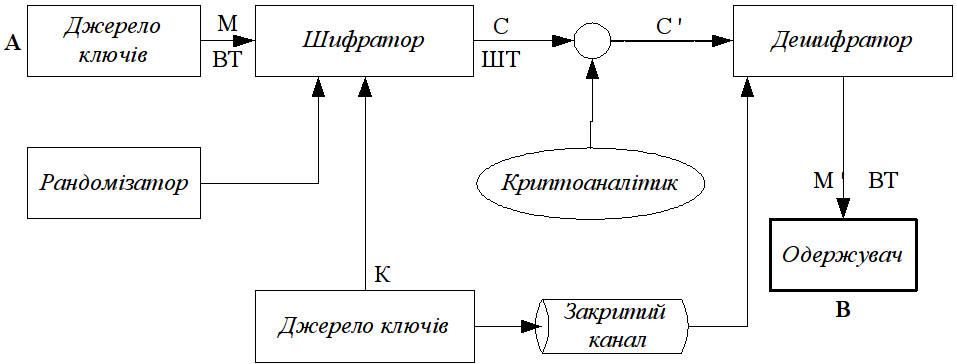
\includegraphics[width=4.0in]{crypt-img/crypt-img4.png}
    \caption{Загальна схема секретного зв'язку}\label{img:secretConnection}
\end{figure}

Розглянемо загальну схему криптографічного захисту зв’язку за допомогою
симетричних криптосистем. Будемо позначати:

$A$ --- відправник;

$B$ --- одержувач;

$M$--- відкритий текст (ВТ);

$C$ --- криптограма (ШТ) відправника;

$C'$ --- отримана криптограма ($C$ може бути змінена при передачі,
наприклад, через перешкоди).

Ключ $k$ заздалегідь передається по закритому
каналу одержувачу (або і відправнику, і одержувачу із джерела ключів), при
цьому неможливо отримати незаконному користувачу ніякої інформації щодо ключа,
здійснити будь-яку зміну в ключі  (вважається, що канал цілком надійний).
Призначення рандомізатора --- використовуючи  зовнішнє джерело випадковості
попередньо зрівняти деякі частотні характеристики ВТ.  Криптоаналітик завжди
може зчитувати ШТ з каналу передачі, але не може змінювати криптограми або мати
якийсь вплив на передачу (так званий пасивний криптоаналітик).

З математичної точки зору криптосистема $\Cryptosystem$ є сукупністю просторів
(множин)
$$\Cryptosystem
    = \left\{ \MessagesSet, \KeysSet, \CryptogramsSet,
        \EAlgorithmsSet, \DAlgorithmsSet \right\}$$

$\MessagesSet$ --- простір всіх повідомлень; $ $

$\KeysSet$ --- простір ключів;

$\CryptogramsSet$ --- простір криптограм;

$\EAlgorithmsSet$ --- простір алгоритмів шифрування;

$\DAlgorithmsSet$ --- простір алгоритмів розшифрування.

Розглянемо  $M, X \in \MessagesSet$ --- деякі повідомлення.
Звичайно повідомлення --- це послідовність букв  деякого алфавіту:
$$M = \left( m_1, \dots, m_n \right),\; X = \left( x_1, \dots, x_n \right)$$

$m_i,x_j$ --- символи ВТ, що є буквами відповідного алфавіту;

$C, Y \in \CryptogramsSet$ --- криптограми, що теж є, як правило, послідовністю
символів деякого алфавіту; 

$k \in \KeysSet$ --- деякий ключ; 

$D_k \in \DAlgorithmsSet$ --- конкретні перетворення (алгоритми) зашифрування і
розшифрування відповідно з ключем $k$. 

У загальному випадку шифр --- це відображення
$$\MessagesSet \times \KeysSet \rightarrow \CryptogramsSet$$

причому
$$\forall k \in \KeysSet,\, \forall M \in \MessagesSet:\;
    D_k\left( E_k\left( M \right) \right) = M,\;
    E_k: \MessagesSet \rightarrow \CryptogramsSet$$

$E_k$ --- ін'єктивне відображення, що дає можливість зашифрувати будь-який ВТ на
ключі $k$.

В теорії Шеннона сформульовані наступні припущення:
\index{Шеннон!припущення}
\begin{enumerate}
    \item Криптоаналітику відомий тільки шифрований текст, тобто атака
        здійснюється на основі шифротексту.
    \item Ключ і рандомізатор використовуються для шифрування тільки один раз
        (тобто криптоаналіз здійснюється тільки по одній криптограмі). 
    \item На  декартовому добутку $\MessagesSet \times \KeysSet$ задано
        ймовірнісний розподіл.
\end{enumerate}

Цей список може бути доповнений новими припущеннями, які Шеннон використовував
неявно, зокрема, такими: канал передачі без спотворень, перетворення
інформації без помилок, відсутній зворотний зв’язок. Хоча вже розроблені більш
загальні теорії, результати Шеннона заклали наріжний камінь криптографії як
науки.

Згідно з правилом Керкгоффса \eqref{def:KerckhoffsPrinciple} всі простори
криптосистеми $\Sigma$ та розподіл на $\MessagesSet \times \KeysSet$ вважаються
відомими криптоаналітику.

Нехай на декартовому добутку $\MessagesSet \times \KeysSet$ задано розподіл
імовірностей 
$$\probability{M, k}:\; \sum_{M, k} \probability{M, k} = 1$$

Зокрема, якщо відкритий текст і ключ, що генеруються, незалежні (а частіше
всього саме так на практиці), то
$$\probability{M, k} = \probability{M} \cdot \probability{k}$$

Цей розподіл $\probability{M, k}$  індукує розподіли ймовірностей на інших
множинах системи. На просторах алгоритмів шифрування $\EAlgorithmsSet$,
алгоритмів розшифрування $\DAlgorithmsSet$ та просторі криптограм
$\CryptogramsSet$ розподіли задаються формулами

\begin{equation}\label{eq:probabilitiesEA}
    \begin{cases}
        \forall k: &\probability{E_k} = \probability{D_k} = \probability{k} \\
        \forall C: &\probability{C}
            = \sum_{\substack{\forall \left( M, k \right):\\
                    E_k\left( M \right) = C}}
                \probability{M, k}
    \end{cases}
\end{equation}

Де останнє підсумовування здійснюється по всіх парах
$\left( M, k \right)$, для яких $E_k\left( M \right) = C$.

Сумісний розподіл ймовірностей криптограм і ключів на
$\CryptogramsSet \times \KeysSet$ задається формулою:

$$\forall \left( C, k \right):\; \probability{C, k}
        = \sum_{\forall M:\;E_k\left( M \right) = C} \probability{M, k}$$


Сумісний розподіл ймовірностей криптограм і відкритих текстів на
$\CryptogramsSet \times \MessagesSet$ індукується наступними співвідношеннями
\begin{equation}\label{eq:jointDistributionMC}
    \forall \left( C, M \right):\; \probability{C, M} = \probability{M, C}
            = \sum_{\forall k:\;E_k\left( M \right) = C} \probability{M, k}
\end{equation}


Ймовірнісні розподіли на вказаних декартових добутках дають можливість знайти
умовні розподіли

$$\begin{array}{lcr}
    \probability{M \mcond C} = \frac{\probability{M, C}}{\probability{C}}, &
    \probability{C \mcond M} = \frac{\probability{M, C}}{\probability{M}}, &
    \probability{k \mcond C} = \frac{\probability{k, C}}{\probability{C}}
\end{array}$$


\section{Цілком таємна (секретна)  криптосистема. Теореми  Шеннона}

Після побудови вищезазначених розподілів можна розглядати також  ентропію множин
з ймовірнісною мірою і побудувати математичну модель криптосистеми. Поняття
цілком таємної криптосистеми формалізує властивість теоретичної стійкості у
теоретико-інформаційному розумінні.

\begin{definition}[Цілком таємна криптосистема]
    Цілком таємною криптосистемою $\Cryptosystem$ називається криптосистема,
    для якої виконується одна з умов
    \begin{enumerate}
        \item\label{item:protectedCS:mc}
            $$\forall M, C:\; \probability{M \mcond C} = \probability{M}$$
        \item\label{item:protectedCS:MC}
            $$\entropyOf{\MessagesSet \mcond \CryptogramsSet}
                = \entropyOf{\MessagesSet}$$
    \end{enumerate}
\end{definition}

\begin{remark}
    Умови \ref{item:protectedCS:mc} і \ref{item:protectedCS:MC} еквівалентні, з
    виконанням однієї умови буде виконуватись і інша.

    Умова \ref{item:protectedCS:mc} означає, що ВТ і ШТ статистично незалежні.

    Умову \ref{item:protectedCS:MC} можна інтерпретувати як відсутність в ШТ
    інформації відносно ВТ, тобто взаємна інформація нульова
    $$I\left( \MessagesSet, \CryptogramsSet \right) = \entropyOf{\MessagesSet}
        - \entropyOf{\MessagesSet \mcond \CryptogramsSet} = 0$$
\end{remark}

\begin{theorem}\label{theorem:protectedCS}
    Необхідною і достатньою умовою цілковитої секретності криптосистеми є
    виконання будь-якої з умов
    \begin{enumerate}
        \item
            $$\forall M, C:\; \probability{C \mcond M} = \probability{C}$$
        \item
            $$\entropyOf{\CryptogramsSet \mcond \MessagesSet}
                = \entropyOf{\CryptogramsSet}$$
    \end{enumerate}
\end{theorem}

\begin{proof}
    Необхідність: якщо система цілком таємна, то 
    $$\probability{M}
        = \probability{M \mcond C}
        =\frac{\probability{M,C}}{\probability{C}}
            \Rightarrow
        \frac{\probability{M,C}}{\probability{M}}
            =\probability{C}
            =\probability{C \mcond M}$$

    Аналогічно доводиться достатність.
\end{proof}

Виникає питання: чи існують цілком таємні криптосистеми? Розглянемо такий
приклад.
\begin{example}[Шифр Вернама (1926 р.)]
    Відкритий текст кодується двійковою послідовністю, ключ та шифртекст також
    представляються послідовностями  ,,$0$'' і ,,$1$'' такої ж довжини.
    ШТ отримується з ВТ і ключа операцією $\mathrm{XOR}$

    $$\begin{array}{lr}

        \begin{array}{r}
            \text{ОТ}: \\
            \text{К}: \\
            \text{ШТ}:
        \end{array} &

        \begin{array}{r}
            \xor
            \begin{array}{r}
                \mathtt{0 1 1 0 1 1 0 1 1 1 0 0 1 0 1} \\
                \mathtt{1 0 1 1 0 1 0 1 0 1 0 1 0 1 1}
            \end{array} \\
            \begin{array}{r}
                \hline
                \mathtt{1 1 0 1 1 0 0 0 1 0 0 1 1 1 0}
            \end{array}
        \end{array}

    \end{array}$$

    У якості ключа береться «ідеально» випадкова послідовність --- послідовність
    незалежних рівноймовірних випадкових біт, тобто кожна реалізація довжини 
    $n$ з‘являється з ймовірністю  $2^{-n}$ незалежно від ВТ. У даному прикладі
    ймовірність появи будь-якої ключової послідовності, а також будь-якої
    криптограми $\frac{1}{2^{15}}$.

    Даний шифр застосовується дотепер (так звана стрічка одноразового
    користування або одноразовий блокнот) на окремих важливих напрямах зв’язку.
    За допомогою побудованої теорії Шеннон довів, що цей шифр є цілком таємним,
    тобто маючи тільки криптограму ніяким чином не можливо знайти відкритий
    текст і навіть будь-яку інформацію щодо нього. Головним недоліком шифра
    Вернама є велика довжина ключа, що треба попередньо передавати по закритому
    каналу. 
\end{example}

\begin{theorem}
    Шифр Вернама є цілком таємною криптосистемою.
\end{theorem}
\begin{proof}
    Маємо відкритий текст
    $$M = m_1 m_2 \dots m_n$$

    Маємо секретний ключ
    $$k = k_1 k_2 \dots k_n$$

    Отримуємо криптограму
    $$C = c_1 c_2 \dots c_n$$

    Все це представлено у вигляді послідовностей бітів
    $$m_i, k_i, c_i \in Z_n = \left\{ 0, 1 \right\}$$

    Використовуємо теорему \ref{theorem:protectedCS}. Безпосередньо за формулою
    \ref{eq:probabilitiesEA} знаходимо ймовірність появи будь-якої криптограми
    $$\forall C: \probability{C}
        = \sum_{\substack{\forall \left( M, k \right):\\
                E_k\left( M \right) = C}} \probability{M, k}
        = 2^{-n} \cdot \sum_{M} \probability{M} = 2^{-n}$$

    Тому що
    $$\probability{M, k}
        = \probability{M} \cdot \probability{k}
        = 2^{-n} \cdot \probability{M}$$

    Далі знайдемо сумісну ймовірність за формулою \ref{eq:jointDistributionMC}
    $$\probability{M, C}
        = \sum_{\forall k:\;E_k\left( M \right) = C} \probability{M, k}
        = 2^{-n} \cdot \probability{M}$$

    Умовна ймовірність
    $$\probability{C \mcond M}
        = \frac{\probability{M, C}}{\probability{M}}
        = \frac{2^{-n} \cdot \probability{M}}{\probability{M}}
        = 2^{-n}$$


    Таким чином, згідно з теоремою \ref{theorem:protectedCS}, шифр Вернама ---
    цілком таємна криптосистема.
\end{proof}

\begin{theorem}[Шеннон]\label{theorem:Shennon}
    Якщо криптосистема цілком таємна, то
    $\entropyOf{\MessagesSet} \le \entropyOf{\KeysSet}$.
    Ця нерівність називається межею Шеннона.
\end{theorem}
\begin{proof}
    Оскільки система цілком таємна, то
    \begin{align*}
        \entropyOf{\MessagesSet}
            = \entropyOf{\MessagesSet \mcond \CryptogramsSet}
            \le \entropyOf{\MessagesSet, \KeysSet \mcond \CryptogramsSet} = \\
            = \entropyOf{\KeysSet \mcond \CryptogramsSet}
                + \entropyOf{\MessagesSet \mcond \KeysSet, \CryptogramsSet}
            = \entropyOf{\KeysSet \mcond \CryptogramsSet}
            \le \entropyOf{\KeysSet}
    \end{align*}

    Тут $\entropyOf{\MessagesSet \mcond \KeysSet, \CryptogramsSet} = 0$, бо при
    відомих ШТ і ключах ВТ однозначно відновлюється. 

    Таким чином, $\entropyOf{\MessagesSet} \le \entropyOf{\KeysSet}$.
\end{proof}

\begin{remark}
    Границя (нерівність) Шеннона є необхідною, але не достатньою умовою
    цілковитої таємності криптосистеми.
\end{remark}

Якщо ключі вибираються рівноймовірно, то ентропія ключів максимальна і дорівнює
довжині ключа в бітах (даного двійковою послідовністю). Для розумного тексту
природною мовою заданого у двійковому алфавіті ентропія дорівнює приблизно
чверті його довжині в бітах. Якби надлишковість дорівнювала нулю, ентропія
такого тексту співпадала б з числом двійкових символів у ньому (дивись лекцію
\ref{lecture:2}). З теореми \ref{theorem:Shennon} випливає, що у цілком таємної
системи при шифруванні тексту великого розміру таємний ключ теж повинен бути
великого розміру (довжини, якщо задається послідовністю символів). І при
зростанні обсягу тексту розмір ключа повинен зростати пропорційно. Таким чином,
криптосистема з фіксованим ключем в загальному випадку не може бути цілком таєм
ою. Для цілковитої таємності секретні ключі для більшості практичних застосуван
мають бути занадто великими. Тому майже усі криптосистеми, що використовуються 
а практиці загалом не є цілком таємними. Вони не мають теоретичної стійкості 
теоретико-інформаційному сенсі й  у принципі можуть бути зламані. Для таких
криптосистем характеристикою їх надійності є практична стійкість. Для не цілком
таємних систем Шеннон розглянув питання теоретико-інформаційної ненадійності, а
також необхідного для зламу шифру обсягу криптограми (це --- тема наступної
лекції).

\section{Контрольні питання}

\begin{enumerate}
    \item Чим відрізняються процедури зашифрування та розшифрування?
    \item Як визначається поняття теоретичної та практичної стійкості
        криптосистеми?
    \item Сформулюйте правило Керкгоффса.
    \item Які припущення зробив Шеннон у запропонованій ним моделі випадкового
        шифру?
    \item Наведіть означення цілком таємної системи в теорії Шеннона.
    \item Що таке границя Шеннона?
    \item Чи виконання нерівності Шеннона є достатньою умовою для цілковитої
        таємності?
    \item Чи існують цілком таємні криптосистеми? 
\end{enumerate}

